%%
%% Author: Dario Chinelli
%% begin 2019-12-04
%% last mod 2022-02-02
%%

% Preamble
\documentclass[class=article, crop=false]{standalone}

% Packages
\usepackage[subpreambles=true]{standalone}
\usepackage{import}
\usepackage{graphicx}
\usepackage{amsmath}

% Document
\begin{document}
% Approximation of path integrals: 3D histogram documentation here
The discrete path integral delineated with the models above is capable of great predictions.
But this structures are hard to represents, moreover the models that includes more than 3 indexes is impossible to represents.
To solve this situation here is used a 3D-histogram.
As histogram this plot express the statistic relevance of a certain data that occurred in dataset.
The 3D space dimensions are: the $x$ direction, the $y$ direction and the $time$ dimension that goes upward.
A 2D surface here represents points in the space-time that have the same occurrence, it's also called \emph{isosurface}.
The following dataset is selected from the Floorfield10 - Utrecht Station.

\subsection{3D comparison between real data and simulations}
In the following results it's distinctive the surface shape, a \emph{tube} isosurface given by the same statistical occurrence.
The shape is the result of a symmetrical distribution around the center of the most probable path.
\\Whats follows doesn't represents the maximum probability nor the minimum, it shows a certain occurrence in the middle that may be useful to compare different datasets.
In this work are considered the \textbf{real data} and the four simulations: \textbf{simD2Q9}, \textbf{simD2Q9Q9}, \textbf{simTD2Q9}, \textbf{simTD2Q9Q9}.
Simulations are generated starting from respectively the four models: \emph{D2Q9}, \emph{D2Q9Q9}, \emph{TD2Q9}, \emph{TD2Q9Q9}.
\\In the figures below are showed the isosurfaces colored by type:
\begin{itemize}
\item BLACK: RealData;
\item LIGHT-BLUE: Simulation D2Q9;
\item PURPLE: Simulation D2Q9Q9;
\item GREEN: Simulation TD2Q9;
\item RED: Simulation TD2Q9Q9.
\end{itemize}

\FloatBarrier
\newpage
\paragraph{Plot of the RealData alone}
In (Figure \ref{fig:comp_RD_1}) and (Figure \ref{fig:comp_RD_2}) it's represented a \emph{tube} surface made from the same statistical occurrence in real data.
\begin{figure}[ht]
\begin{minipage}[c]{0.5\linewidth}
\centering
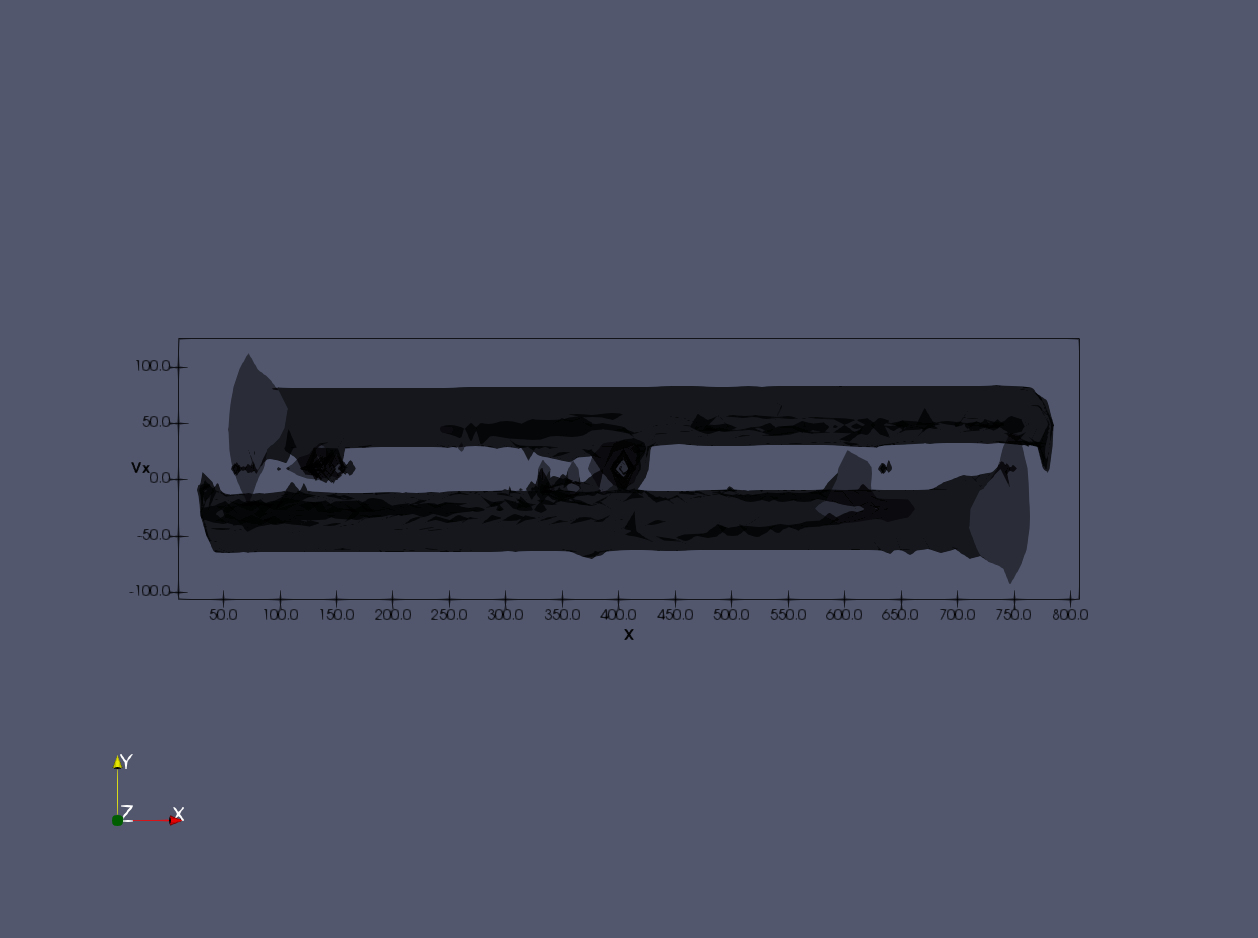
\includegraphics[ width=.9\textwidth]{fig/3d-hist/trainf10_X_Vx_RealData}
\captionsetup{width=.81\linewidth}
\caption{Real data. Top view: where the time direction is pointing out of the plot, it's clearly visible the shape along the spaces directions.}
\label{fig:comp_RD_1}
\end{minipage}
\begin{minipage}[c]{0.5\linewidth}
\centering
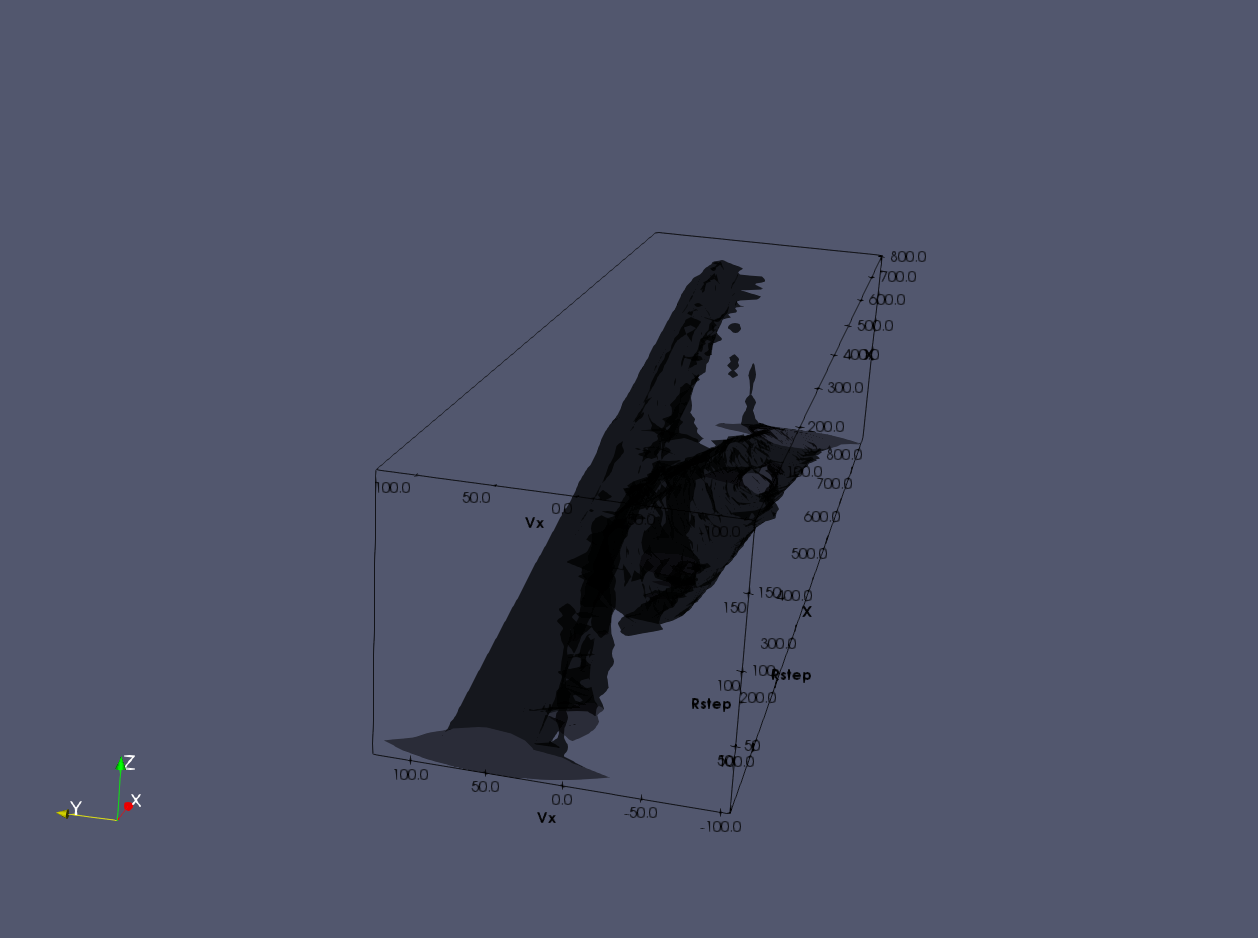
\includegraphics[ width=.9\textwidth]{fig/3d-hist/trainf10_X_Vx_RealData-2}
\captionsetup{width=.81\linewidth}
\caption{Real data. Side view: it's possible to distinguish the three dimensions. The shape goes UP in time and move horizontally in space.}
\label{fig:comp_RD_2}
\end{minipage}
\end{figure}

\FloatBarrier
\paragraph{Comparison between RealData and Simulations}
The following 8 figures, from (Figure \ref{fig:comp_RD_D2Q9_1} - \ref{fig:comp_RD_TD2Q9Q9_2}), show the same statistical occurrence in datasets.
From the first to the last model it's over and over clearer the good overlay between the simulation and the real data.
For the firsts two models is pretty difficult to see a good overlaying, even if it's not null.
For the lasts two models is easy to see the improve made by adding the \emph{time} information.

\begin{figure}[ht]
\begin{minipage}[c]{0.5\linewidth}
\centering
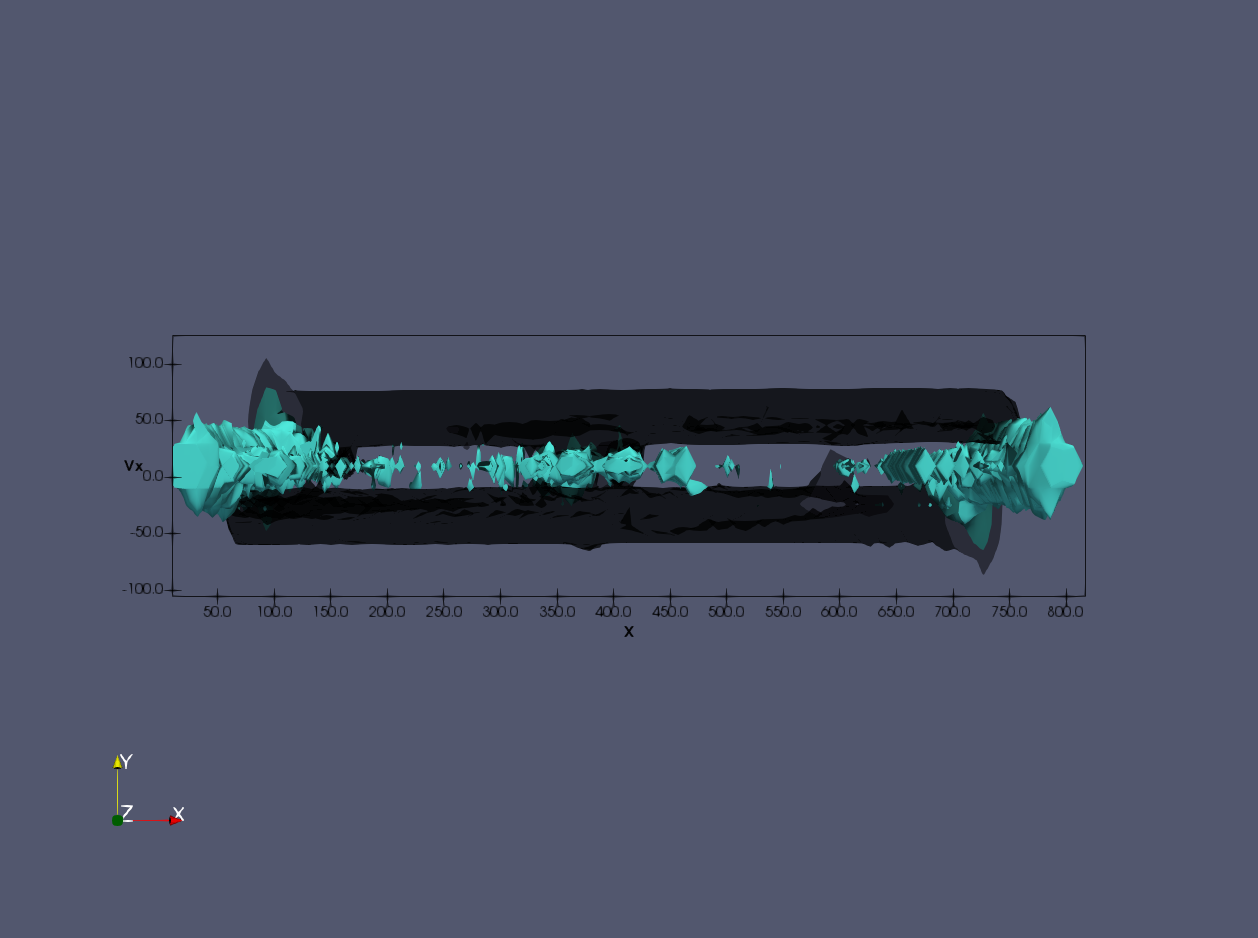
\includegraphics[ width=.9\textwidth]{fig/3d-hist/trainf10_X_Vx_RealData_and_simD2Q9}
\captionsetup{width=.81\linewidth}
\caption{Top view: model D2Q9 in light blue and real data in black.}
\label{fig:comp_RD_D2Q9_1}
\end{minipage}
\begin{minipage}[c]{0.5\linewidth}
\centering
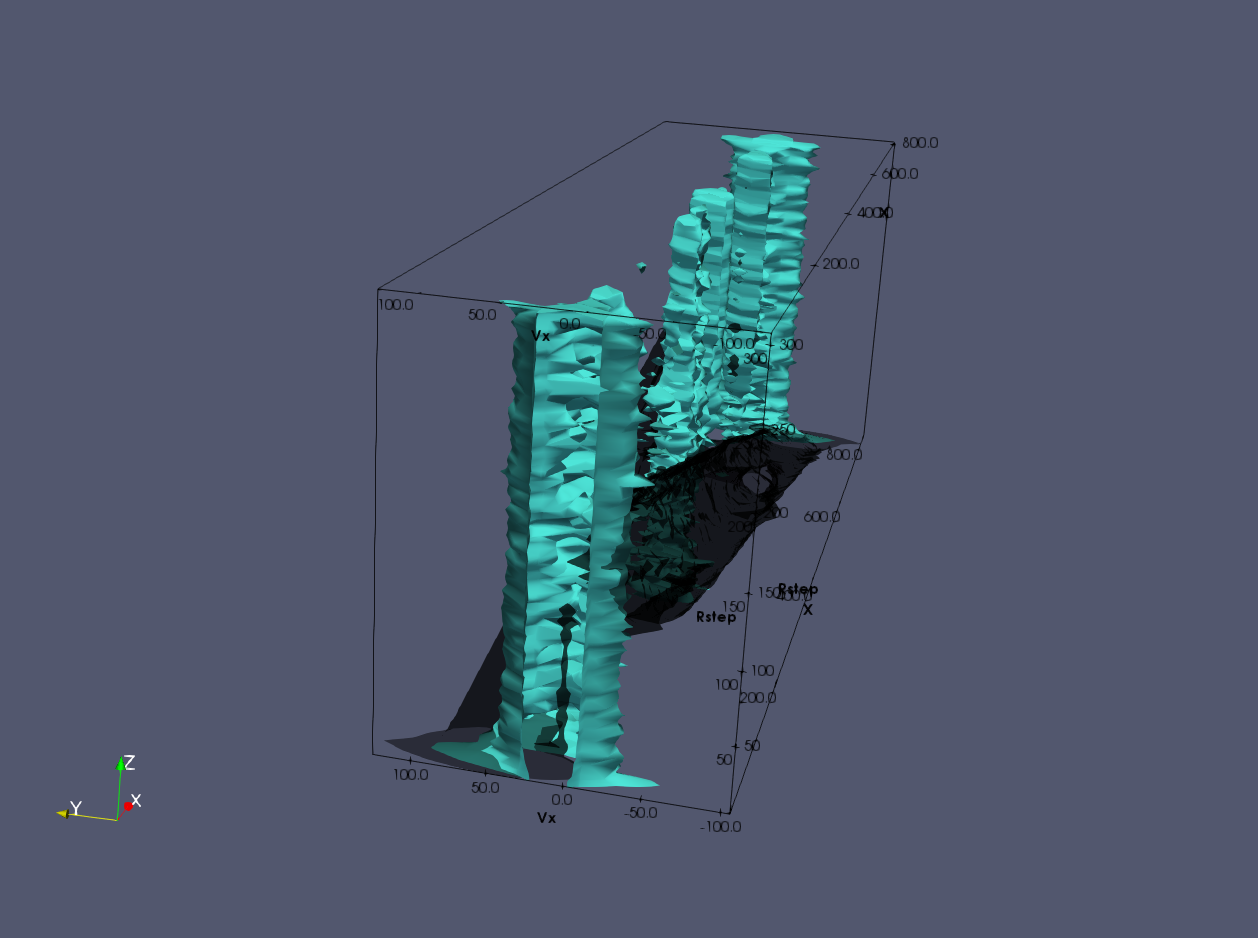
\includegraphics[ width=.9\textwidth]{fig/3d-hist/trainf10_X_Vx_RealData_and_simD2Q9-2}
\captionsetup{width=.81\linewidth}
\caption{Side view: model D2Q9 in light blue and real data in black.}
\label{fig:comp_RD_D2Q9_2}
\end{minipage}

\begin{minipage}[c]{0.5\linewidth}
\centering
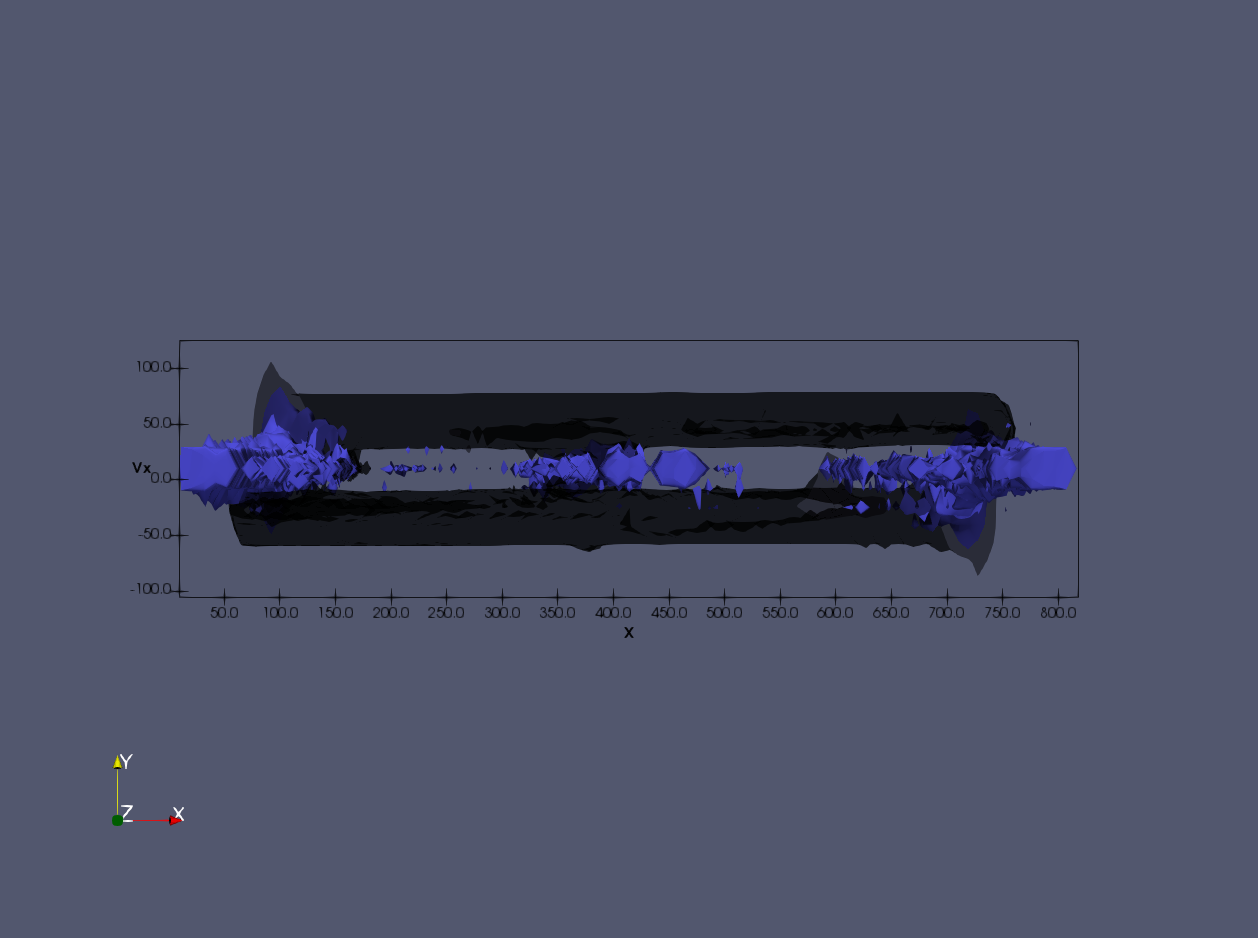
\includegraphics[ width=.9\textwidth]{fig/3d-hist/trainf10_X_Vx_RealData_and_simD2Q9Q9}
\captionsetup{width=.81\linewidth}
\caption{Top view: model D2Q9Q9 in purple and real data in black.}
\label{fig:comp_RD_D2Q9Q9_1}
\end{minipage}
\begin{minipage}[c]{0.5\linewidth}
\centering
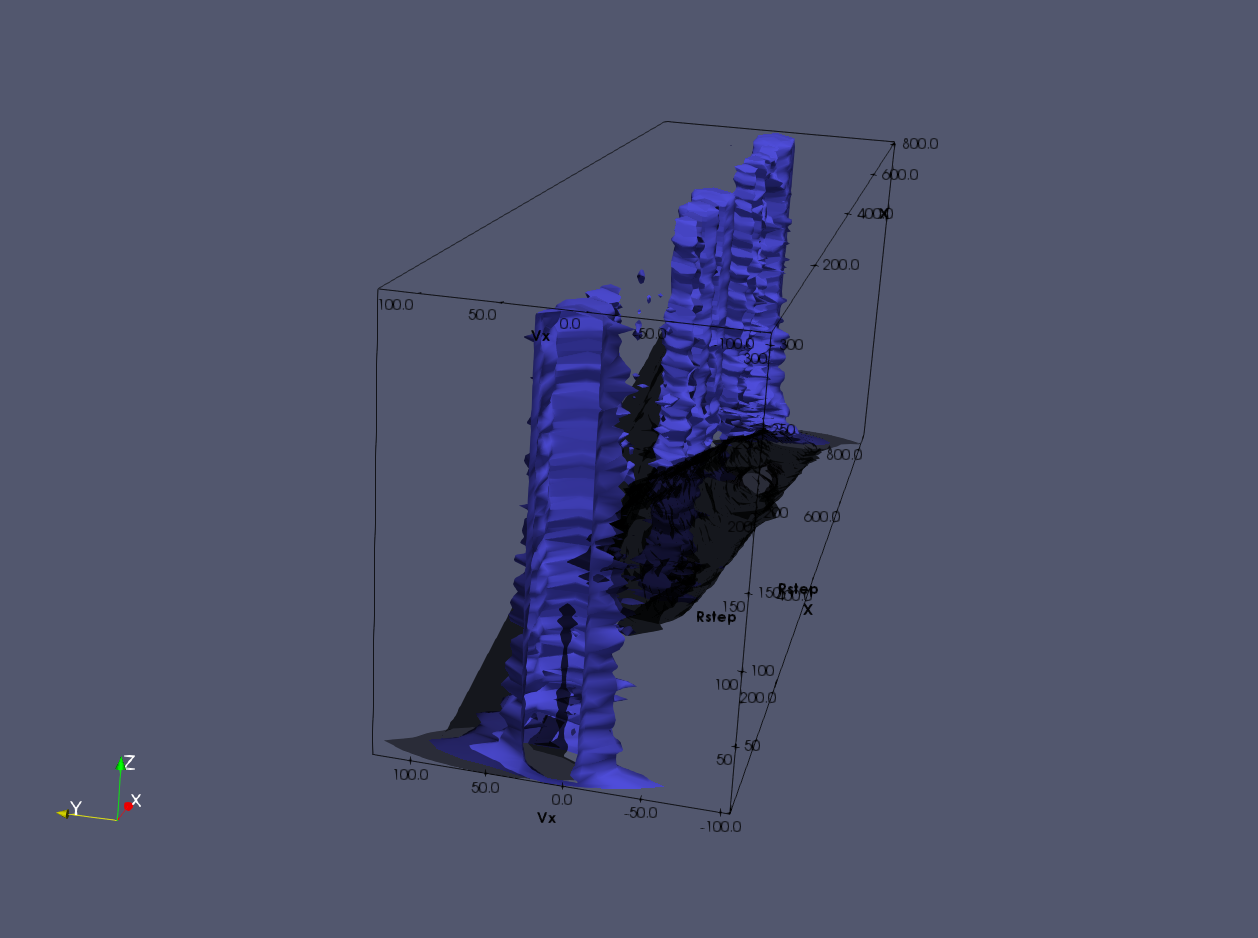
\includegraphics[ width=.9\textwidth]{fig/3d-hist/trainf10_X_Vx_RealData_and_simD2Q9Q9-2}
\captionsetup{width=.81\linewidth}
\caption{Side view: model D2Q9Q9 in purple and real data in black.}
\label{fig:comp_RD_D2Q9Q9_2}
\end{minipage}

\begin{minipage}[c]{0.5\linewidth}
\centering
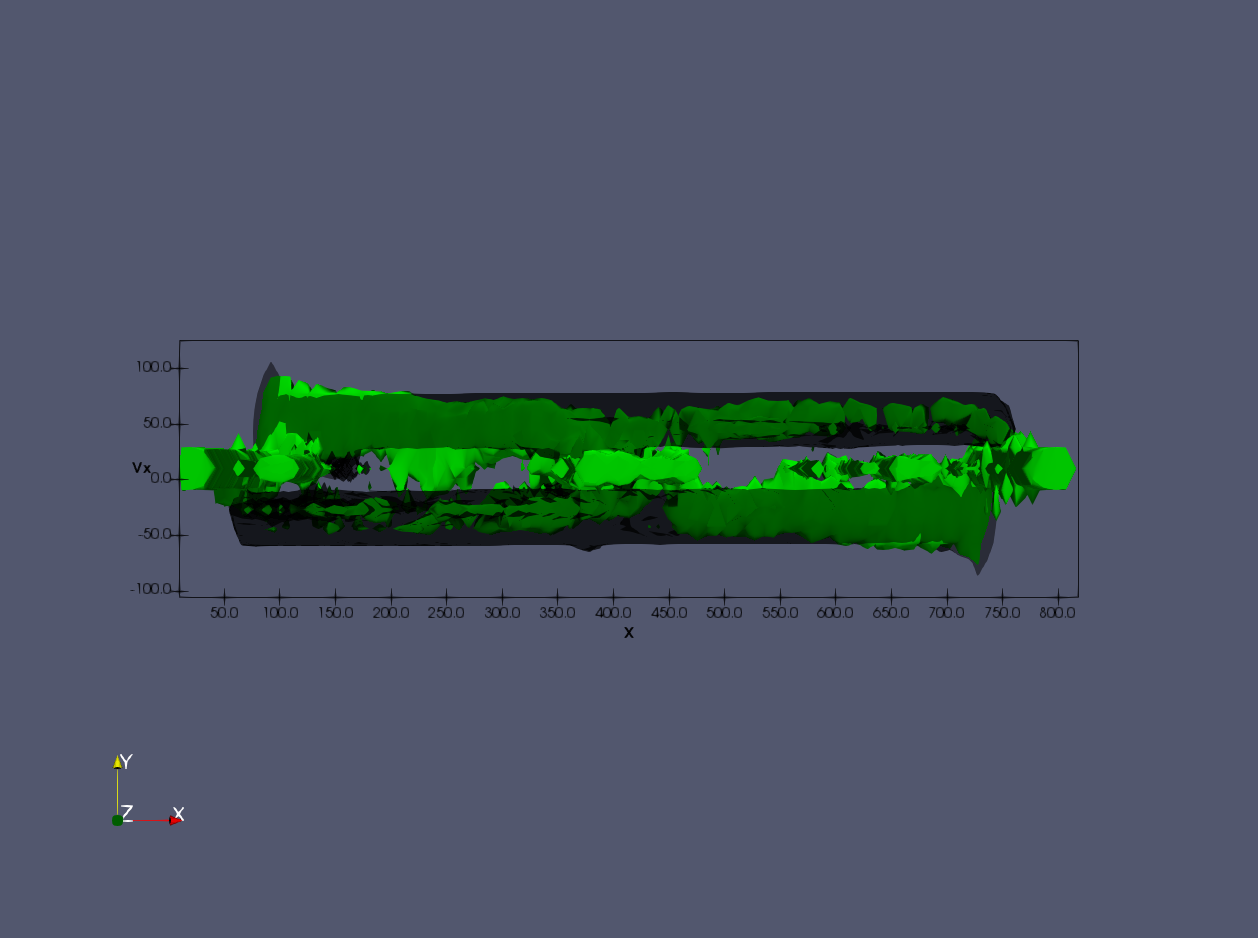
\includegraphics[ width=.9\textwidth]{fig/3d-hist/trainf10_X_Vx_RealData_and_simTD2Q9}
\captionsetup{width=.81\linewidth}
\caption{Top view: model TD2Q9 in green and real data in black.}
\label{fig:comp_RD_TD2Q9_1}
\end{minipage}
\begin{minipage}[c]{0.5\linewidth}
\centering
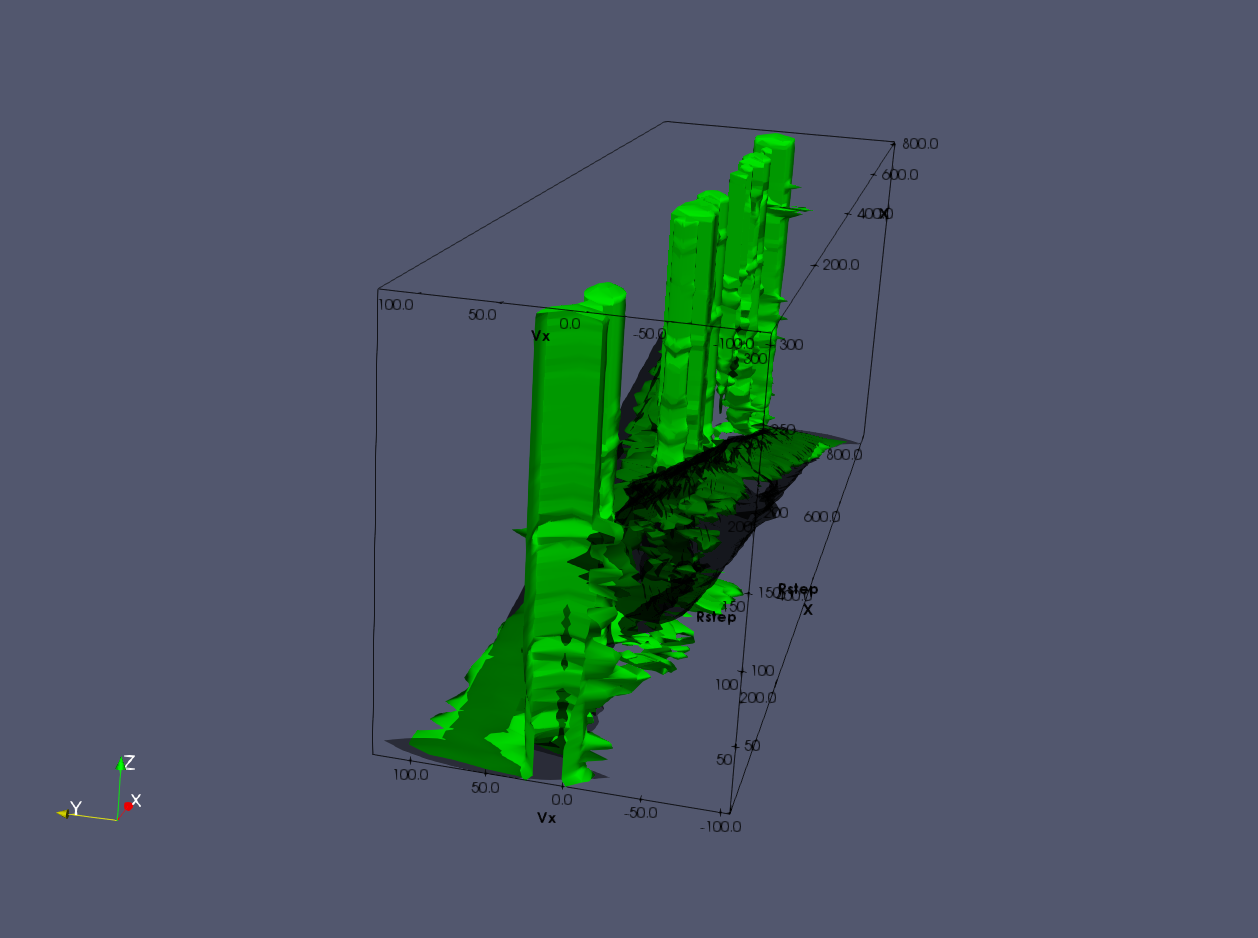
\includegraphics[ width=.9\textwidth]{fig/3d-hist/trainf10_X_Vx_RealData_and_simTD2Q9-2}
\captionsetup{width=.81\linewidth}
\caption{Side view: model TD2Q9 in green and real data in black.}
\label{fig:comp_RD_TD2Q9_2}
\end{minipage}

\begin{minipage}[c]{0.5\linewidth}
\centering
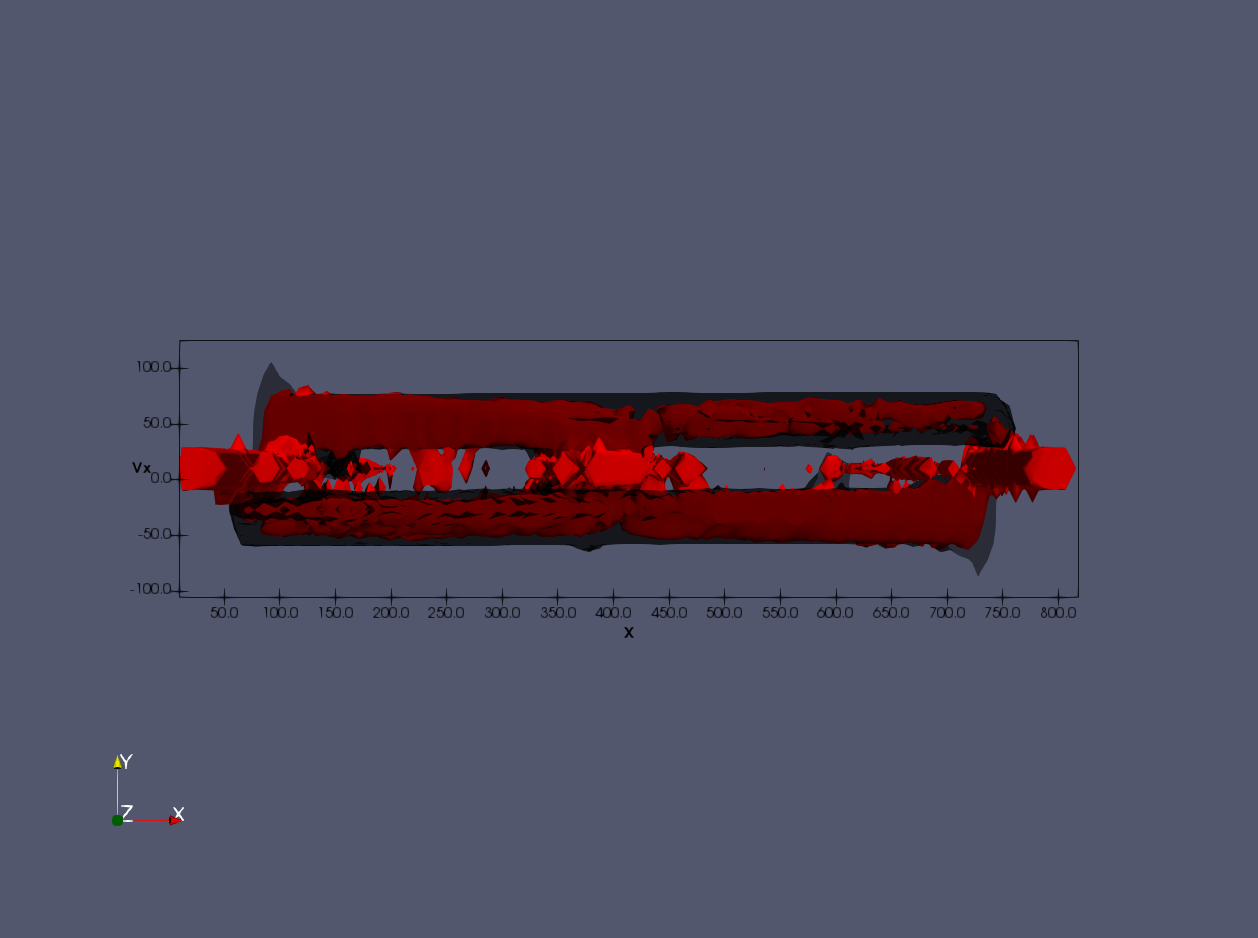
\includegraphics[ width=.9\textwidth]{fig/3d-hist/trainf10_X_Vx_RealData_and_simTD2Q9Q9}
\captionsetup{width=.81\linewidth}
\caption{Top view: model TD2Q9Q9 in red and real data in black.}
\label{fig:comp_RD_TD2Q9Q9_1}
\end{minipage}
\begin{minipage}[c]{0.5\linewidth}
\centering
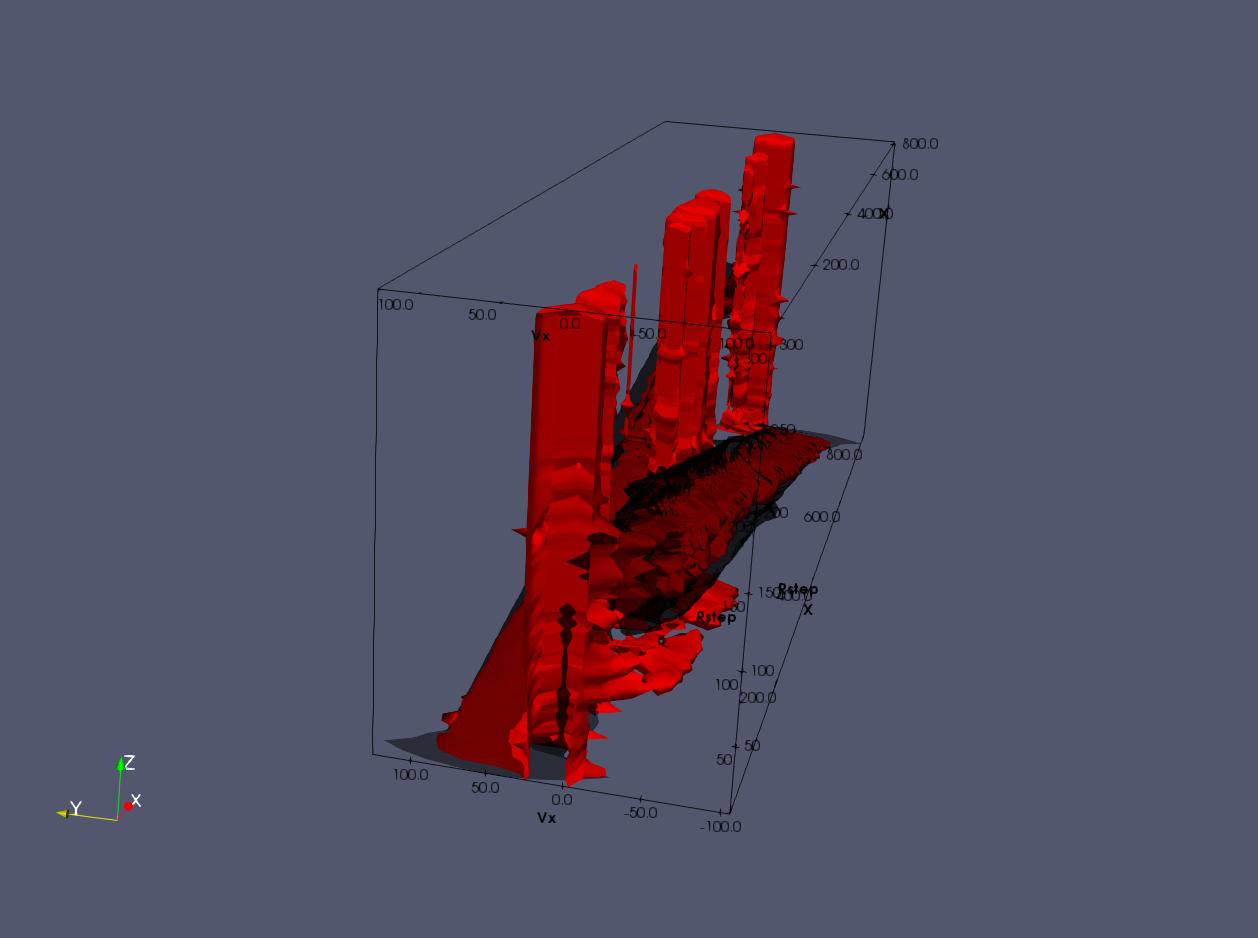
\includegraphics[ width=.9\textwidth]{fig/3d-hist/trainf10_X_Vx_RealData_and_simTD2Q9Q9-2}
\captionsetup{width=.81\linewidth}
\caption{Side view: model TD2Q9Q9 in red and real data in black.}
\label{fig:comp_RD_TD2Q9Q9_2}
\end{minipage}
\end{figure}





\FloatBarrier
\end{document}
